\subsection{Bandstruktur}
\begin{frame}
\frametitle{Bandstruktur}
\begin{minipage}{0.7\textwidth}
\begin{figure}
	\centering
	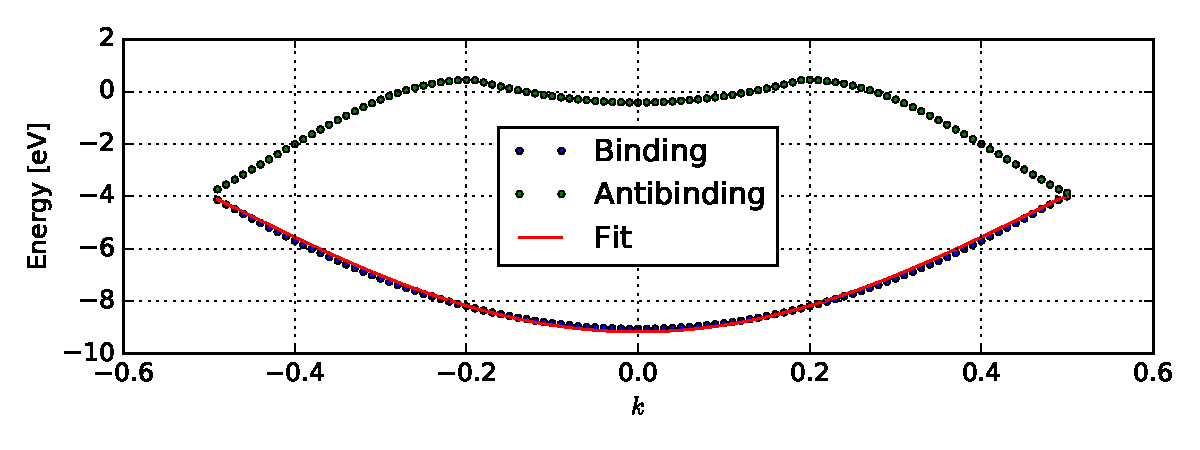
\includegraphics[width = \textwidth]{Images/polyacetylene/bandstructure/band_fit}\\
	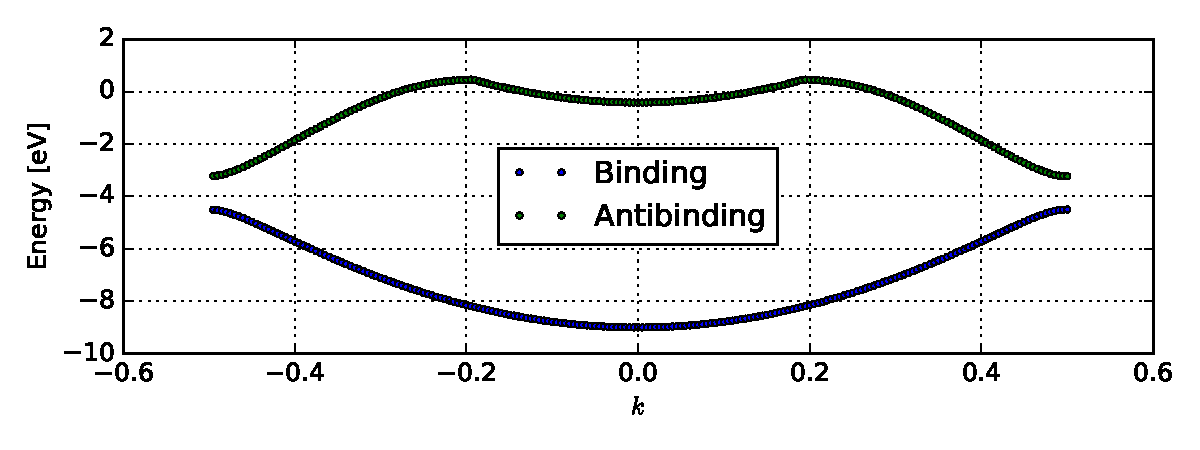
\includegraphics[width = \textwidth]{Images/polyacetylene/bandstructure/band_manually_displaced}
	\caption{Bandstruktur \emph{trans}-Polyacetylen}
	\label{image_band_structure_relaxed_polyacetylene}
\end{figure}
\end{minipage}
\begin{minipage}{.29\textwidth}
\begin{itemize}
\setlength\itemsep{.2cm}
\item Berechnet:\\
$t_0 = \unit[2.62]{eV}$\\
Literaturwert:\\
$t_0 = \unit[2.5]{eV}$
\item Berechnet:\\
$E_\text{Gap} = \unit[0.14]{eV}$\\
$\hspace*{1.15cm}(\unit[1.27]{eV})$\\
Literaturwert:\\
$E_\text{Gap} = \unit[1.4]{eV}$
\item Berechnet:\\
$\alpha = \unit[3.95]{eV/\AA}$\\
Literaturwert:\\
$\alpha = \unit[4.1]{eV/\AA}$
\end{itemize}
\end{minipage}
\end{frame}


\section{Dichtefunktionaltheorie mit Zwangsbedingungen}
\subsection{Motivation}
\begin{frame}
\frametitle{Motivation für neuen Ansatz}
Direkte Auswertung der Bandstruktur oft schwierig
\vspace*{.5cm}

\centering
\begin{tikzpicture}[]
\foreach \i in {0,1,...,5}{
	\draw (2*\i, 0) circle (.2);};
\draw[->] (5.8, .2) .. controls (5.5, .7) and (4.5, .7) .. (4.2, .2) node [midway, above] {$t$};
\draw [fill = blue] (5.79, .21) circle (.07);
\draw [dotted, line width = 1] (10.3, 0) -- +(.3, 0);
\draw [dotted, line width = 1] (-0.3, 0) -- +(-.3, 0);

\begin{axis}[
no markers, domain=0:10, samples=100,
xtick=\empty, ytick=\empty,
height=4cm, width=6.5cm, hide axis,
at = {(2.55cm, -1.2cm)}
]
\addplot [dashed, cyan!50!black, domain = 3:4.95] {-.5 * gauss(4,.3)};
\addplot [dashed, cyan!50!black, domain = 5.05:7] {.5*gauss(6,.3)};
\end{axis}
\end{tikzpicture}
\vspace*{.5cm}
\begin{align*}
\mathcal{H}_\text{hopp} &= - \sum_i t_{i, i+1} \left(c_i^\dagger\  c_{i+1} + c_{i+1}^\dagger\  c_i\right)
\end{align*}
\end{frame}

\begin{frame}{Dichtefunktionaltheorie mit Zwangsbedingungen (cDFT)}
\hspace*{-.5cm}
\begin{minipage}{0.75\textwidth}
	\vspace*{-1.5cm}
	\begin{itemize}
		\item Manuelles Verschieben von Ladung mittels externen Potentialen
		\item Definiere $i$ Regionen und Ladungen $N_i$
		\item Überlagerte Gauß-Kurven $w(\vec{r})$ zentriert an Kernpositionen $\vec{R}_j$
	\end{itemize}
\end{minipage}
\begin{minipage}{0.25\textwidth}
	\vspace*{-.8cm}
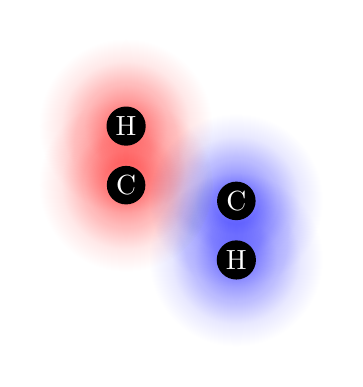
\begin{tikzpicture}[scale = 0.5]
	\foreach \i/\j/\color in {0/0.2/red, 0/1.7/red, 2.8/-0.2/blue, 2.8/-1.7/blue}{
		\foreach \r in {0, 0.01, ..., 1}{
			\fill[opacity = \r * 0.017, fill = \color] (\i, \j) circle ({2.5 * (1 - \r)});}}
	\foreach \i/\j/\num in {0/0.2/C, 0/1.7/H, 2.8/-0.2/C, 2.8/-1.7/H}{
		\node[fill = black, shape = circle, text = white, inner sep = 0.05cm] at (\i, \j)	 {\num};}
\end{tikzpicture}
\end{minipage}
\hspace*{-.5cm}
\begin{minipage}{\textwidth}
\vspace*{-1cm}
\begin{itemize}
	\item Minimierung der cDFT-Energie:
	\begin{align*}
	F\left[n\left(\vec{r}\right), U_i\right] &= E_0\left[n\left(\vec{r}\right)\right] + 
	\sum_i U_i\left(\int\dd\vec{r}\ w_i\left(\vec{r}\right)\ n\left(\vec{r}\right) - N_i\right)
	\end{align*}
	mit den Zwangsbedingungen:
	\begin{align*}
	0 &= \int\dd\vec{r}\ w_i\left(\vec{r}\right)\ n\left(\vec{r}\right) - N_i
	\end{align*}
\end{itemize}
\end{minipage}
\end{frame}

\begin{frame}
\frametitle{Kette von Wasserstoff-Atomen}
\begin{minipage}{0.6\textwidth}
Möglichst einfaches Testsystem für cDFT
\end{minipage}
\begin{minipage}{0.39\textwidth}
\centering
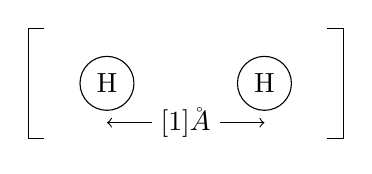
\begin{tikzpicture}
\node [circle, draw] at (0,0) {H};
\node [circle, draw] at (2,0) {H};
\draw (-0.8, 0.7) -- ++(-0.2, 0) -- ++(0, -1.4) -- ++(.2, 0);
\draw (2.8, 0.7) -- ++(0.2, 0) -- ++(0, -1.4) -- ++(-.2, 0);
\draw [<->] (0, -.5) -- +(2, 0) node [midway, fill = white] {$\small\unit[1]{\AA}$};
\end{tikzpicture}
\end{minipage}
\begin{figure}[]
	\centering
	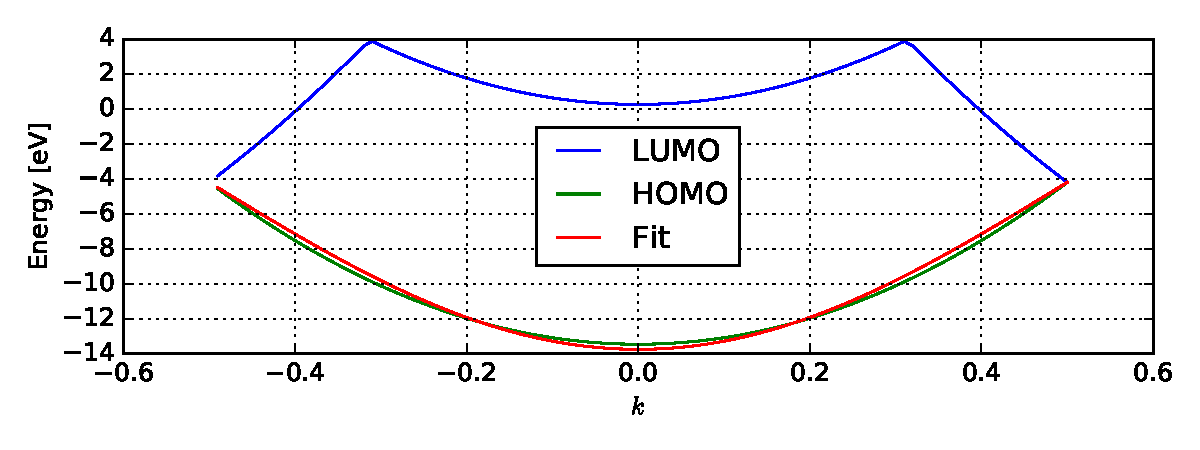
\includegraphics[width = 9cm]{Images/Hydrogen/bands/hydrogen_band_structure}
	\caption{Bandstruktur der Wasserstoff-Kette}
	\label{image_hydrogen_band_structure}
\end{figure}
\centering
$\Rightarrow\quad t_0 = \unit[4.8]{eV}$ 
\end{frame}

\begin{frame}
\frametitle{Korrektur von cDFT mit periodischen Randbedingungen}
\begin{figure}
\centering
\begin{subfigure}{0.45\textwidth}
\centering
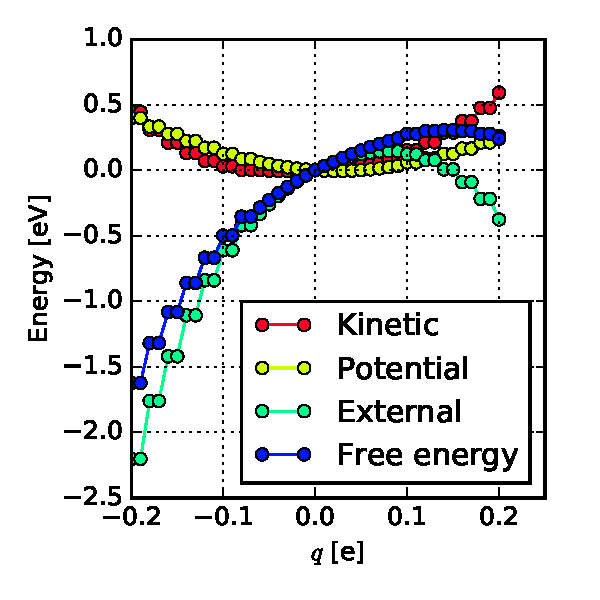
\includegraphics[width = \textwidth]{Images/Hydrogen/charging/energy_contributions_asymmetric}
\caption{Verschiedene Energiebeiträge zur Gesamtenergie in Abhängigkeit von der verschobenen Ladung $q$.}
\label{image_contributions_initial}
\end{subfigure}\hspace*{1cm}
\begin{subfigure}{0.45\textwidth}
\centering
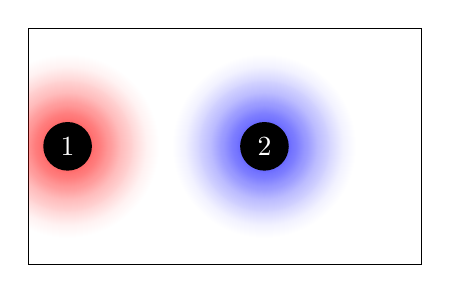
\begin{tikzpicture}[]
\begin{scope}
\clip [draw] (-.5, -1.5) rectangle (4.5, 1.5);
\foreach \x/\color in {0/red, 2.5/blue}{
\foreach \r in {0, 0.01, ..., 1}{
\fill[opacity = \r * 0.03, fill = \color] (\x, 0) circle ({2.5 * (.5 - 0.5 * \r)});}}
\foreach \x/\num in {0/1, 2.5/2}{
\node[fill = black, shape = circle, text = white] at (\x, 0)	 {\num};}
\end{scope}
\end{tikzpicture}
\caption{Schema: \textsc{Gauß}-Kurven mit periodischer Randbedingung.}
\end{subfigure}
\end{figure}
\end{frame}

\begin{frame}
\begin{figure}
\centering
\begin{subfigure}{0.45\textwidth}
\centering
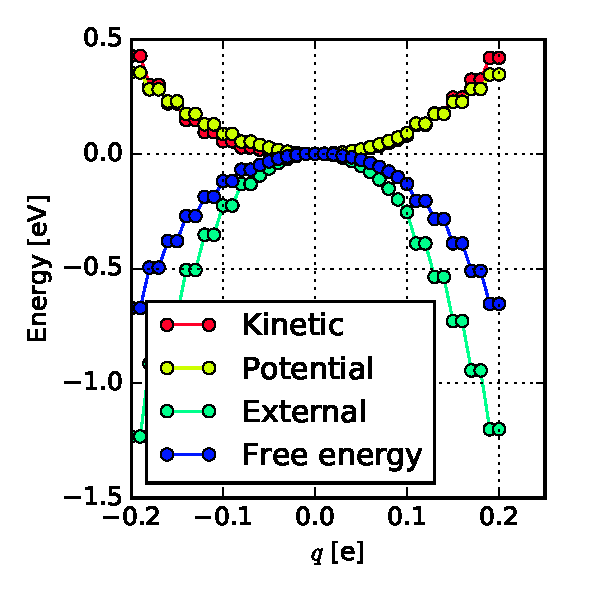
\includegraphics[width = \textwidth]{Images/Hydrogen/charging/energy_contributions_symmetric}
\caption{Verschiedene Energiebeiträge zur Gesamtenergie in Abhängigkeit von der verschobenen Ladung $q$.}
\label{image_contributions_corrected}
\end{subfigure}\hspace*{1cm}
\begin{subfigure}{0.45\textwidth}
\centering
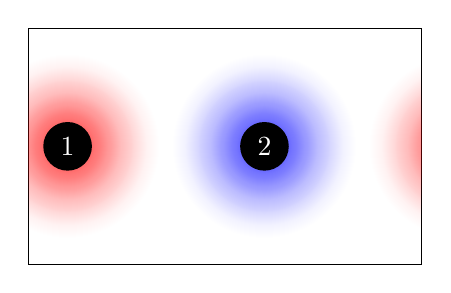
\begin{tikzpicture}
\begin{scope}
\clip [draw] (-.5, -1.5) rectangle (4.5, 1.5);
\foreach \x/\color in {0/red, 2.5/blue, 5/red}{
\foreach \r in {0, 0.01, ..., 1}{
\fill[opacity = \r * 0.03, fill = \color] (\x, 0) circle ({2.5 * (.5 - 0.5 * \r)});}}
\foreach \x/\num in {0/1, 2.5/2}{
\node[fill = black, shape = circle, text = white] at (\x, 0)	 {\num};}
\end{scope}
\end{tikzpicture}
\caption{Schema: Korrigierte \textsc{Gauß}-Kurven mit periodischer Randbedingung.}
\end{subfigure}
\end{figure} 
\end{frame}

\subsection{Erstes Modell zur Beschreibung der Ladungsverschiebung}
\begin{frame}
\frametitle{Erstes Modell zur Beschreibung der Ladungsverschiebung}
\begin{itemize}
\setlength{\itemsep}{.8cm}
\item Hopping-Hamiltonian unverändert
\item Wellenfunktionen einheitlich variieren:
\begin{align*}
\Psi_k^{(v)}(q) &= \sqrt{\frac{1}{2}-\frac{q}{2}}c_k^{\dagger(e)}- \sqrt{\frac{1}{2}+\frac{q}{2}}c_{k}^{\dagger(o)}
\end{align*}
\item Grundzustandsenergie als Summe der Einteilchen-Energien:
\begin{align*}
E_0(q) &= -\frac{8t_0}{\pi} \sqrt{1-q^2}
\end{align*}
\end{itemize}
\end{frame}

\begin{frame}
\frametitle{Standardabweichung der \textsc{Gauß}-Kurven}
\begin{itemize}
\item Zu kleines $\sigma\quad\Rightarrow\quad$ Lokalisiert Elektronen zu sehr
\item Zu großes $\sigma\quad\Rightarrow\quad$ Ungezielte Verschiebung
\item $\sigma$ mit leichtest möglicher Ladungsverschiebung
\end{itemize}
\begin{figure}[!t]
	\centering
	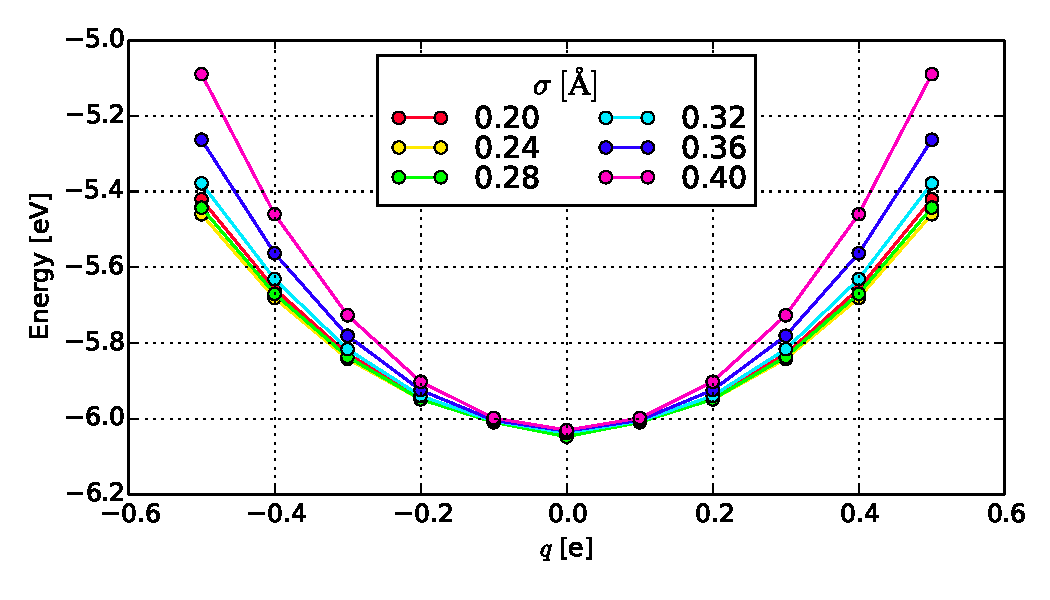
\includegraphics[width = 7.5cm]{Images/Hydrogen/charging/gaussian_sigmas}
	\caption{Grundzustandsenergie in Abhängigkeit von der verschobenen cDFT Ladung für verschiedene $\sigma$.}
	\label{image_gaussian_sigmas_hydrogen}
\end{figure}
\end{frame}

\begin{frame}
\frametitle{Berechnung des Hopping-Parameters}
\begin{minipage}{0.49\textwidth}
\begin{align*}
E_0(q) &= -\frac{8t_0}{\pi} \sqrt{1-q^2}
\end{align*}
\begin{itemize}
\setlength{\itemsep}{.5cm}
\item Ergebnis: $t_0 = \unit[9.0]{eV}$
\item Referenzwert: $t_0 = \unit[4.8]{eV}$
\end{itemize}
\end{minipage}
\begin{minipage}{0.49\textwidth}
\begin{figure}
\centering
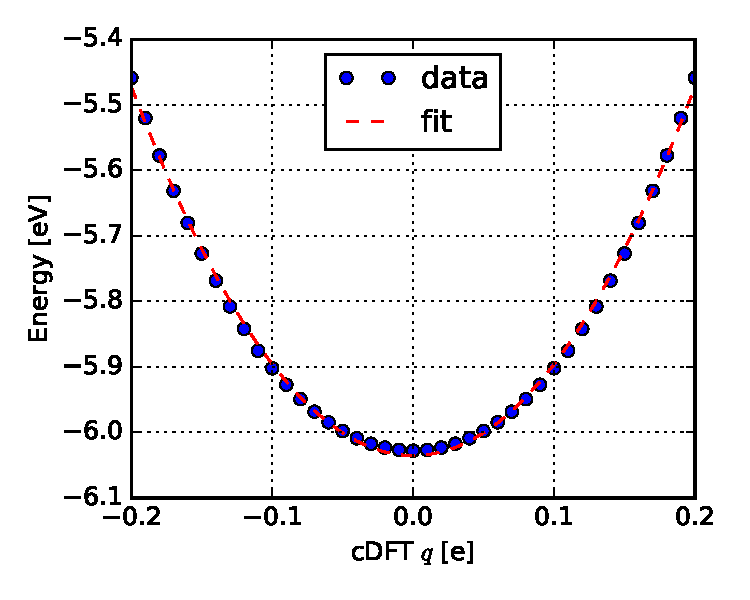
\includegraphics[width = \textwidth]{Images/Hydrogen/charging/energy_fit_normal_sigma}
\caption{Grundzustandsenergie in Abhängigkeit der verschobenen Ladung für $\sigma = \unit[0.24]{\AA}$}
\label{}
\end{figure}
\end{minipage}
\end{frame}

\begin{frame}
Ursachen:
\begin{itemize}
\item Grundzustandsenergie $\neq$ Summe Einteilchen-Energien
\item $E_k$ variieren nicht gleichmäßig
\end{itemize}
\begin{figure}
\centering
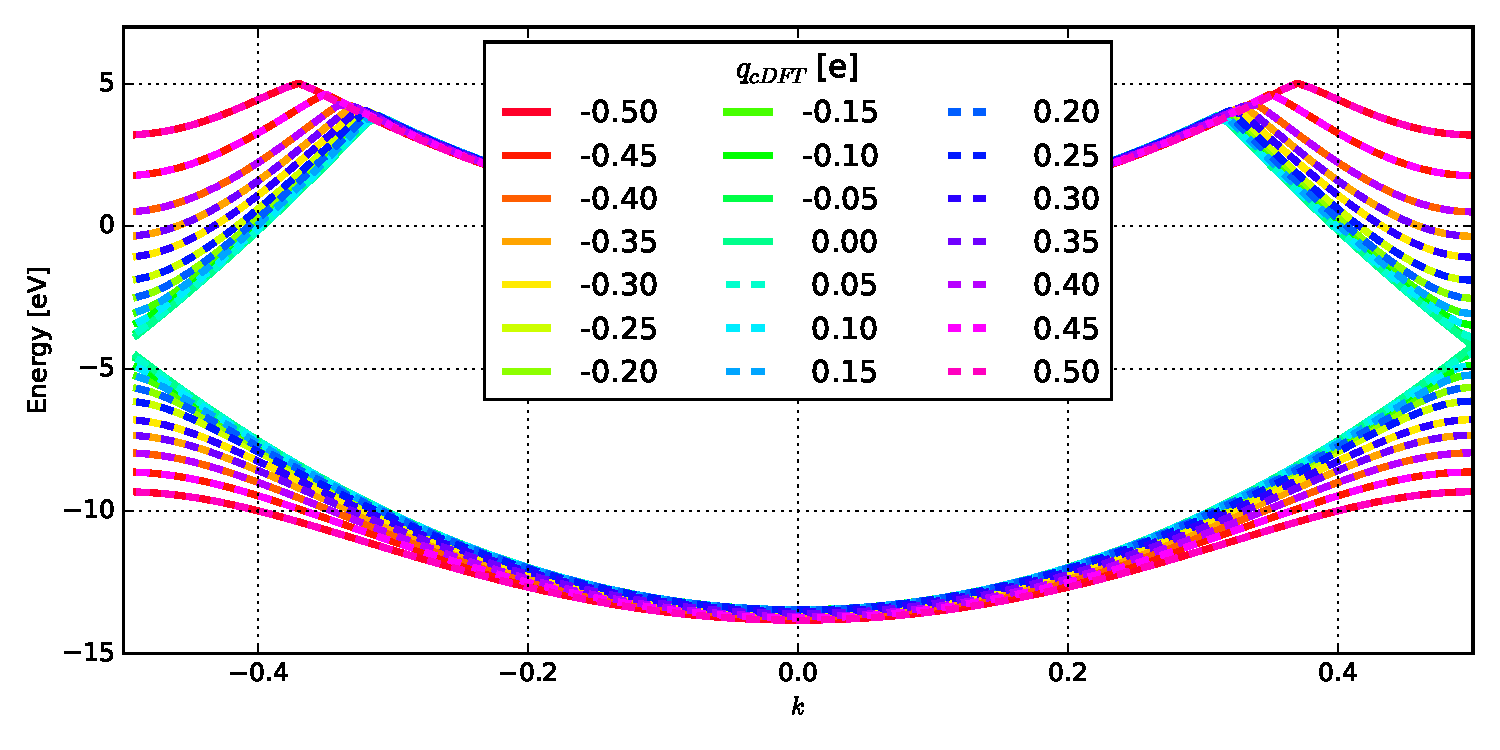
\includegraphics[width = 11cm]{Images/Hydrogen/charging/band_structure_q_1}
\caption{HOMO- and LUMO-Band für verschiedene Ladungsverschiebungen.}
\label{image_hydrogen_charged_bands}
\end{figure}
\end{frame}

\subsection{Zweites Modell zur Beschreibung der Ladungsverschiebung}
\begin{frame}
\frametitle{Zweites Modell zur Beschreibung der Ladungsverschiebung}
\begin{itemize}
\setlength{\itemsep}{.5cm}
\item Modifiziere Hopping-Hamiltonian:
\begin{align*}
\begin{pmatrix*}[c]
0 & \epsilon_k + i \Delta_k \\
\epsilon_k - i \Delta_k & 0
\end{pmatrix*} 
&\to 
\begin{pmatrix*}[c]
-V & \epsilon_k + i \Delta_k \\
\epsilon_k - i \Delta_k & V
\end{pmatrix*}
\end{align*}
\item Mit Eigenwerten:
\begin{align*}
E_k = \pm \sqrt{V^2+\epsilon_k^2+\Delta_k^2}
\end{align*}
\item Für Wasserstoff-Kette ($\Delta_k = 0$):
\begin{align*}
E_k &= \pm \sqrt{V^2 + \left(2t_0\cos(ka)\right)^2}
\end{align*}
\end{itemize}
\end{frame}

\begin{frame}
\begin{figure}
\centering
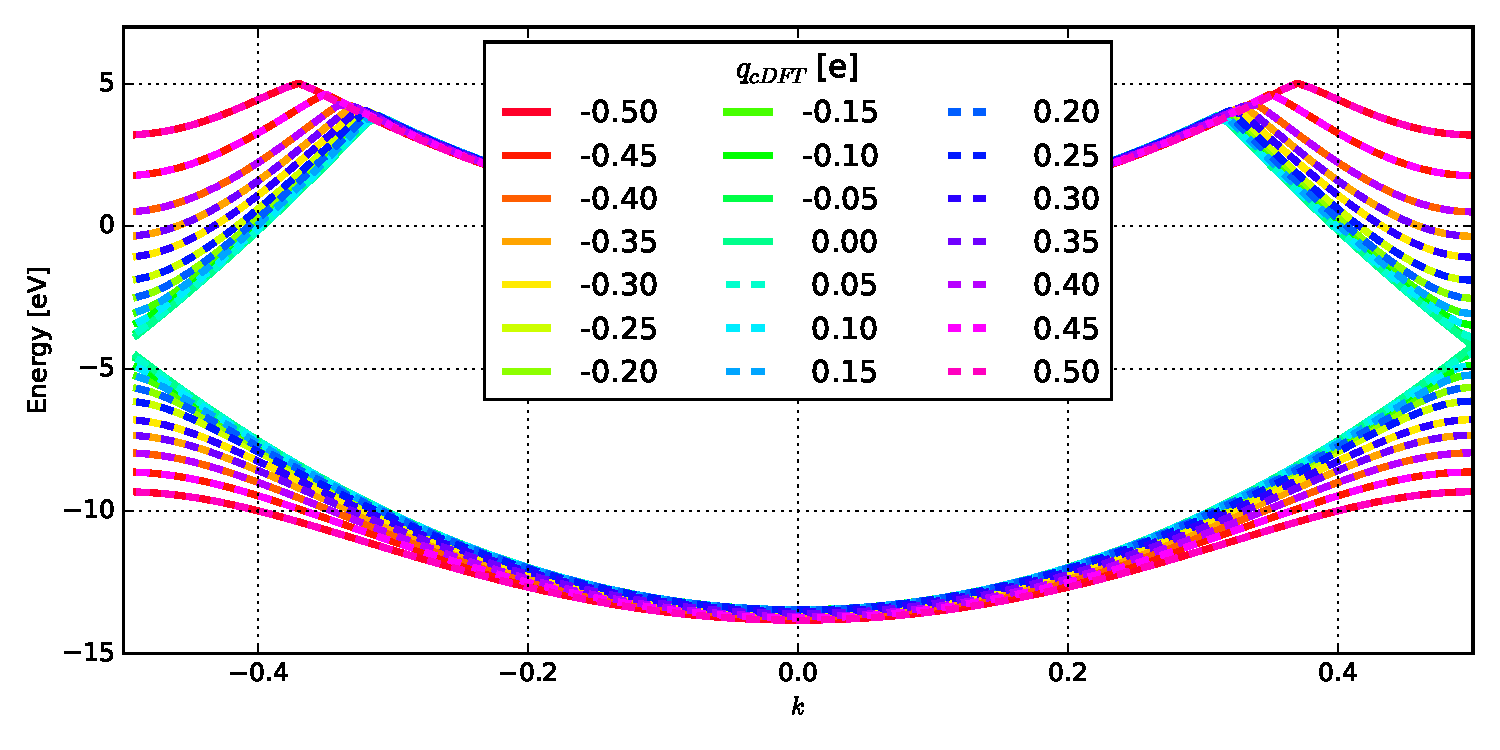
\includegraphics[width = 11cm]{Images/Hydrogen/charging/band_structure_q_1}
\caption{HOMO- and LUMO-Band für verschiedene Ladungsverschiebungen.}
\label{image_hydrogen_charged_bands}
\end{figure}
\begin{align*}
E_k &= \pm \sqrt{V^2 + \left(2t_0\cos(ka)\right)^2}
\end{align*}
\end{frame}

\begin{frame}
\begin{minipage}{0.49\textwidth}
\begin{itemize}
\setlength{\itemsep}{1cm}
\item $V$ korrespondiert mit cDFT Potential-Stärken $U_i$
\item Erwartung von Hamiltonian:
\begin{align*}
U_1 = -U_2
\end{align*}
\item $V = c \cdot U$\\
$U = \frac{1}{2}(U_1 - U_2)$
\end{itemize}
\end{minipage}
\begin{minipage}{0.49\textwidth}
\begin{figure}
\centering
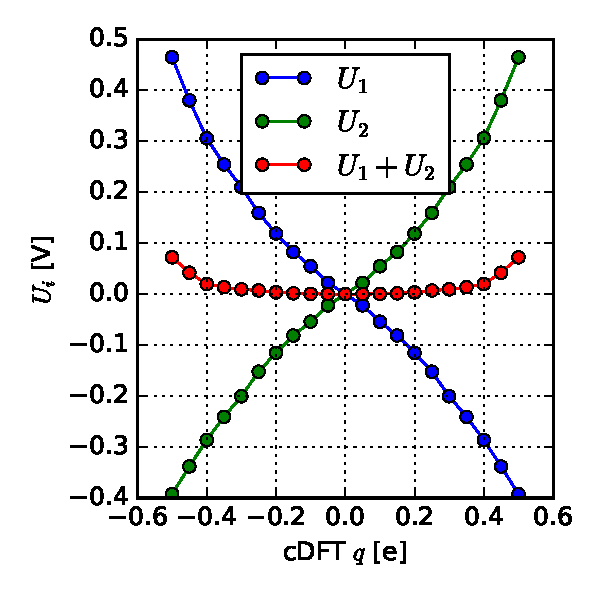
\includegraphics[width = \textwidth]{Images/Hydrogen/charging/potential_q_1}
\caption{cDFT potentials in respect to the displaced charge.\\}
\label{image_potentials_qs_1}
\end{figure}	
\end{minipage}
\end{frame}

\begin{frame}
\begin{figure}[]
	\centering
	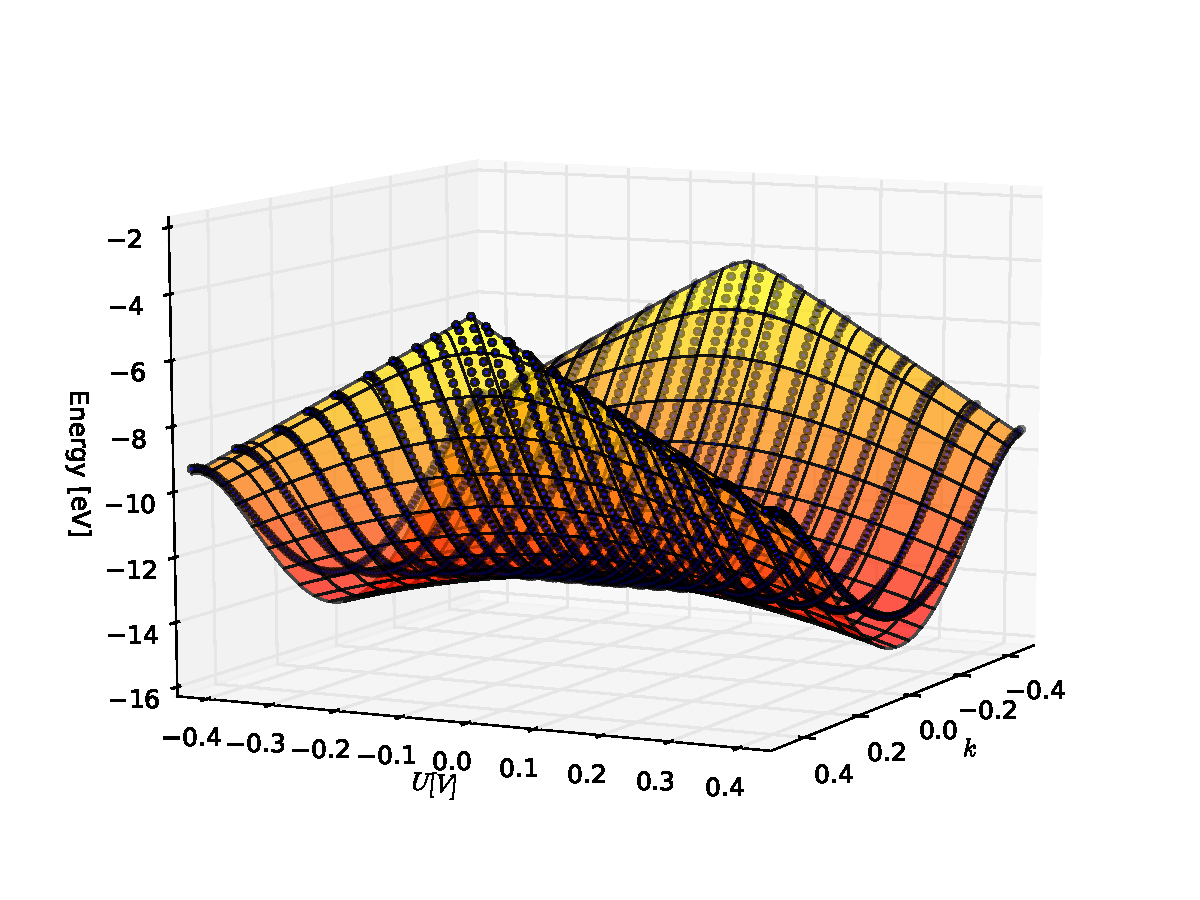
\includegraphics[width = .8\textwidth]{Images/Hydrogen/charging/3D/figure_1-1}
\end{figure}
\begin{minipage}{0.5\textwidth}
\begin{itemize}
\item Fit: $\hspace*{1.6cm} t_0 = \unit[4.6]{eV}$
\item Referenzwert: $t_0 = \unit[4.8]{eV}$
\end{itemize}
\end{minipage}
\begin{minipage}{0.49\textwidth}
\begin{align*}
E_k &= \pm \sqrt{(cU)^2 + \left(2t_0\cos(ka)\right)^2}
\end{align*}
\end{minipage}
\end{frame}

\begin{frame}
\frametitle{Zweites Modell für \emph{trans}-Polyacetylen}
\begin{figure}
\begin{subfigure}{0.3\textwidth}
\centering
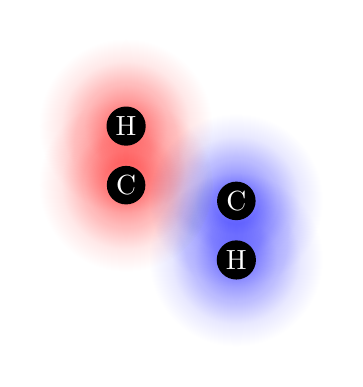
\begin{tikzpicture}[scale = 0.5]
	\foreach \i/\j/\color in {0/0.2/red, 0/1.7/red, 2.8/-0.2/blue, 2.8/-1.7/blue}{
		\foreach \r in {0, 0.01, ..., 1}{
			\fill[opacity = \r * 0.017, fill = \color] (\i, \j) circle ({2.5 * (1 - \r)});}}
	\foreach \i/\j/\num in {0/0.2/C, 0/1.7/H, 2.8/-0.2/C, 2.8/-1.7/H}{
		\node[fill = black, shape = circle, text = white, inner sep = 0.05cm] at (\i, \j)	 {\num};}
\end{tikzpicture}
\end{subfigure}
\begin{subfigure}{0.68\textwidth}
\centering
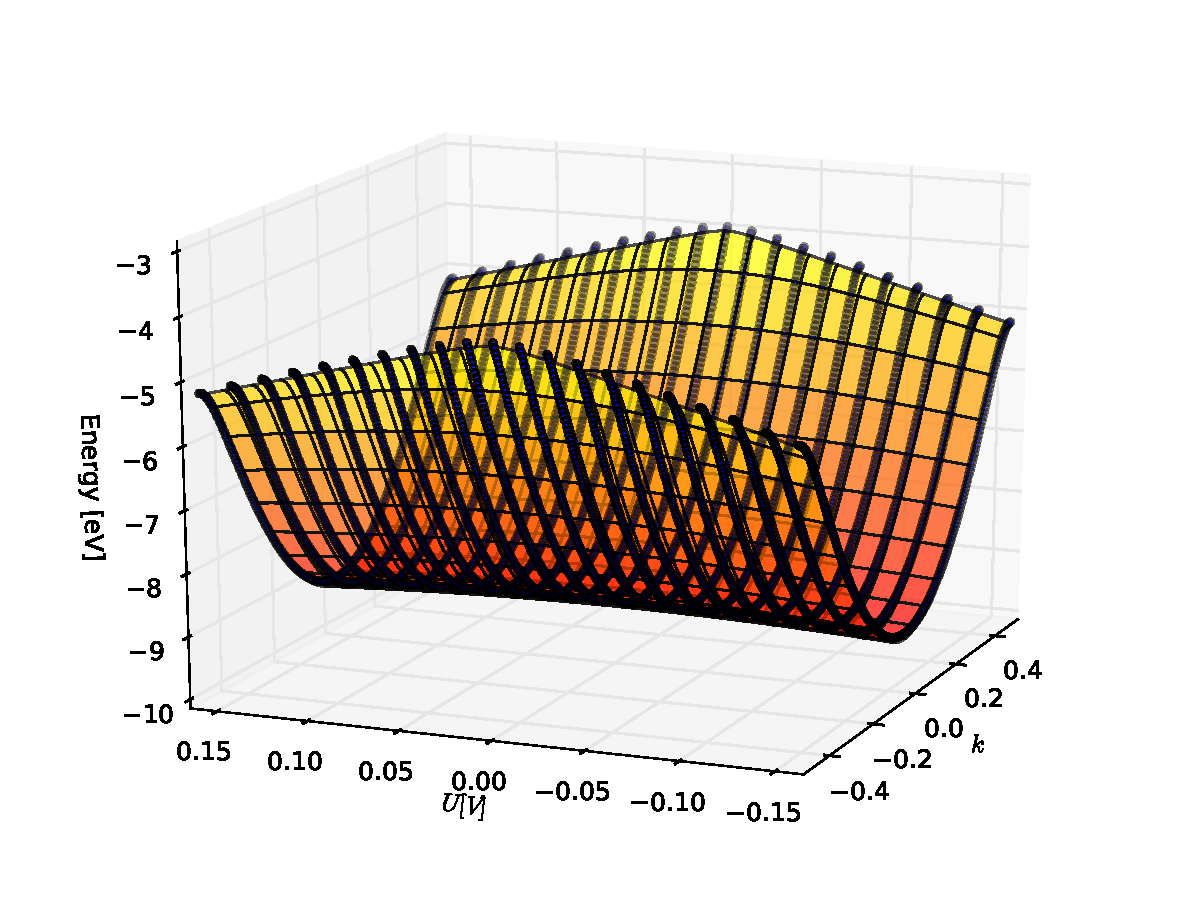
\includegraphics[width = \textwidth]{Images/polyacetylene/charging/3D/figure_1-2}
\end{subfigure}
\end{figure}
\begin{itemize}
\item Fit: $\hspace*{1.6cm}t_0 = \unit[2.6]{eV}$
\item Referenzwert: $t_0 = \unit[2.6]{eV}$
\end{itemize}
\end{frame}

\begin{frame}
\begin{minipage}{0.64\textwidth}
\begin{figure}
	\centering
	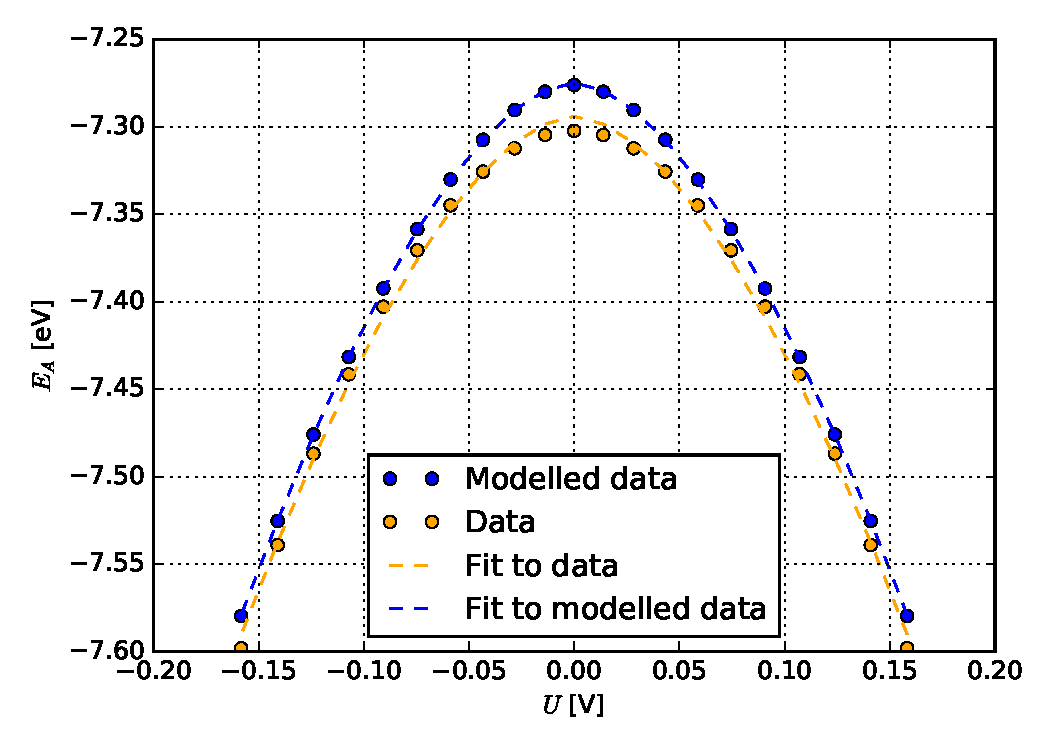
\includegraphics[width = \textwidth]{Images/polyacetylene/charging/Homo_energy_charge}
	\caption{Mittlere HOMO-Band-Energie in Abhängigkeit von $U$.}
	\label{image_HOMO_average_polyacetylene}
\end{figure}
\end{minipage}
\begin{minipage}{0.34\textwidth}
\begin{itemize}
\setlength{\itemsep}{1cm}
\item Modellierte Daten: $t_0 = \unit[2.6]{eV}$
\item Simulations Daten: $t_0 = \unit[2.7]{eV}$
\end{itemize}
\end{minipage}
$E_A(V) = \frac{-2}{\pi}\sqrt{V^2+4t_0^2}\int\limits_0^{\nicefrac{\pi}{2}}\dd\theta\sqrt{1-\xi^2\cdot\sin^2(\theta)}\qquad$
mit $\xi^2 = \frac{4t_0^2 - 4\delta^2}{V^2+4t_0^2}$

\end{frame}


\section{Zusammenfassung}
\begin{frame}
\frametitle{Zusammenfassung}
Gute Bandstruktur mit DFT
\begin{table}[!h]
	\centering
	\begin{tabular}{l|c|c}
		Größe & Berechnet & Lit.\\
		\hline \hline
		&&\\[-.3cm]
		Bindungslänge \hfill$a [\unit{\AA}]$ & $1.23$ & $1.2$\\ \hline&&\\[-.3cm]
		Verschiebung \hfill$u [\unit{\AA}]$& $0 - 5\cdot10^{-3}$ & $0.042$\\ \hline&&\\[-.3cm]
		Bandlücke \hfill$E_\text{Gap} [\unit{eV}]$ & $0.137\quad(1.27)$ & $1.4$\\ \hline &&\\[-.3cm]
		Hopping-Parameter \hfill$t_0 [\unit{eV}]$ & $2.62$ & $2.5$ \\ \hline&&\\[-.3cm]
		Phonon-Kopplungs-Konstante \hspace*{.5cm}$\alpha [\unitfrac{eV}{\AA}]$& $3.95$ & $4.1$
	\end{tabular}
\end{table}
'Proof of Principle': Hopping-Parameter aus Ladungsverschiebung (cDFT)\\
\begin{align*}
t_0 = \unit[2.7]{eV}
\end{align*}
\end{frame}

\begin{frame}
\centering
\begin{huge}
Vielen Dank für Ihre Aufmerksamkeit
\end{huge}

\end{frame}